\documentclass[11pt]{jsarticle}
\usepackage[dvipdfmx]{graphicx}
\graphicspath{ {images/} }
\usepackage{wrapfig}
\usepackage{ascmac}
\usepackage{geometry}
\usepackage[hypertex]{hyperref}
\usepackage[dvipdfmx]{color}
\def\red#1{{\color{red}{#1}}}

\usepackage{fancyhdr}
\geometry{body={160mm,230mm},columnsep=8mm}

\usepackage{listings}
%%%% Jun
\usepackage{listings,jlisting}
\lstset{
  language=c,
  basicstyle=\ttfamily\small,
  commentstyle=\textit,
  classoffset=1,
  keywordstyle=\bfseries,
  numbers=left,stepnumber=1,
%  frame=tRBI,
  frame=single,
  framesep=5pt
  }

\usepackage{makeidx} %索引
\makeindex

\makeatletter
\newcounter{qnum}[section]
\setcounter{qnum}{0}
\def\theqnum{問\thesection.\the\c@qnum}
\def\question{\refstepcounter{qnum}%
  \vspace{3mm}\noindent\textbf{[\theqnum]}~}

\newcounter{wnum}[section]
\setcounter{wnum}{0}
\def\thewnum{課題\thesection.\the\c@wnum}
\def\work{\refstepcounter{wnum}%
  \vspace{3mm}\noindent\textbf{[\thewnum]}~}

\def\waku#1#2{\begin{itembox}[l]{\bf #1}#2\end{itembox}}

%%% index
\def\bfindex{\@ifnextchar[{\@bfindex}{\@@bfindex}}
\def\@bfindex[#1]#2{\textbf{#2}\index{#1@#2}}
\def\@@bfindex#1{\textbf{#1}\index{#1}}

\def\nmindex{\@ifnextchar[{\@nmindex}{\@@nmindex}}
\def\@nmindex[#1]#2{#2\index{#1@#2}}
\def\@@nmindex#1{#1\index{#1}}
\makeatother

%\def\question{\noindent\textbf {[問題]}}
%\newenvironment{vscreen}{\begin{screen}\begin{verbatim}}{\end{verbatim}\end{screen}}


\begin{document}
\pagestyle{empty}
\vspace{-0.6cm}
\noindent
\rule{\linewidth}{0.5pt}
\begin{center}
{\Large LEGO MindStorm EV3のRobotCによる制御プログラミング}
\end{center}
\begin{flushright}
\today 版\\
西井 淳
\end{flushright}
\vspace{-0.6cm}
\rule{\linewidth}{0.5pt}

\vspace{-0.6cm}
% \newpage
{\small
  \setcounter{tocdepth}{3}
  \tableofcontents
}

\newpage
\pagestyle{fancy}
%\def\baselinestretch{1.02}


\begin{wrapfigure}[8]{r}{5.5cm}\vspace{-.5cm}
  \resizebox{5.5cm}{!}{\includegraphics{robotc_default.eps}}
  \caption{\label{fig:start}RobotCの起動画面}
\end{wrapfigure}
\section{はじめに}

\subsection{LEGO MindStormとRobotCについて}
\nmindex{LEGO MindStorm}\index{MindStorm}はLEGOがMITと共同開発したロボット制御の学習用キットです。
本テキストでは,LEGO MindStorm EV3をプログラミング言語\nmindex{RobotC}
を使って制御する方法を説明します。
RobotCでは,3種類のプログラムスタイルを利用できますが,演習では
Text-Based ROBOTC Commandsと呼ばれるC言語と似た言語を使います。

\begin{wrapfigure}[18]{r}{5cm}\vspace{-.5cm}
{\small
\centering
\resizebox{5cm}{!}{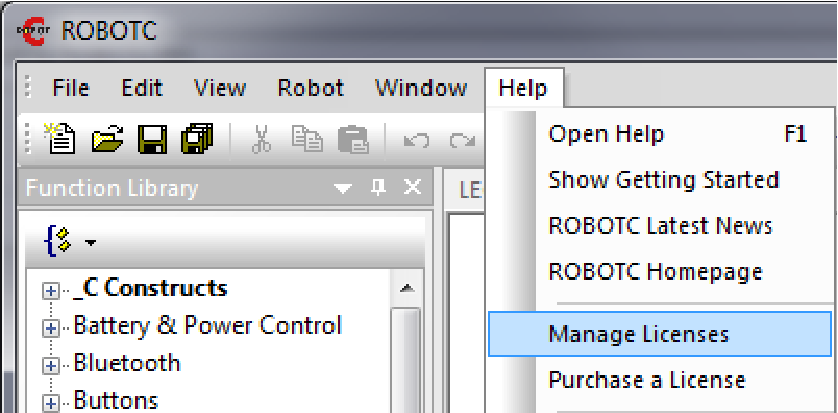
\includegraphics{1-manage-license.pdf}}\\
(1) ライセンス認証メニュー選択\\
\resizebox{5cm}{!}{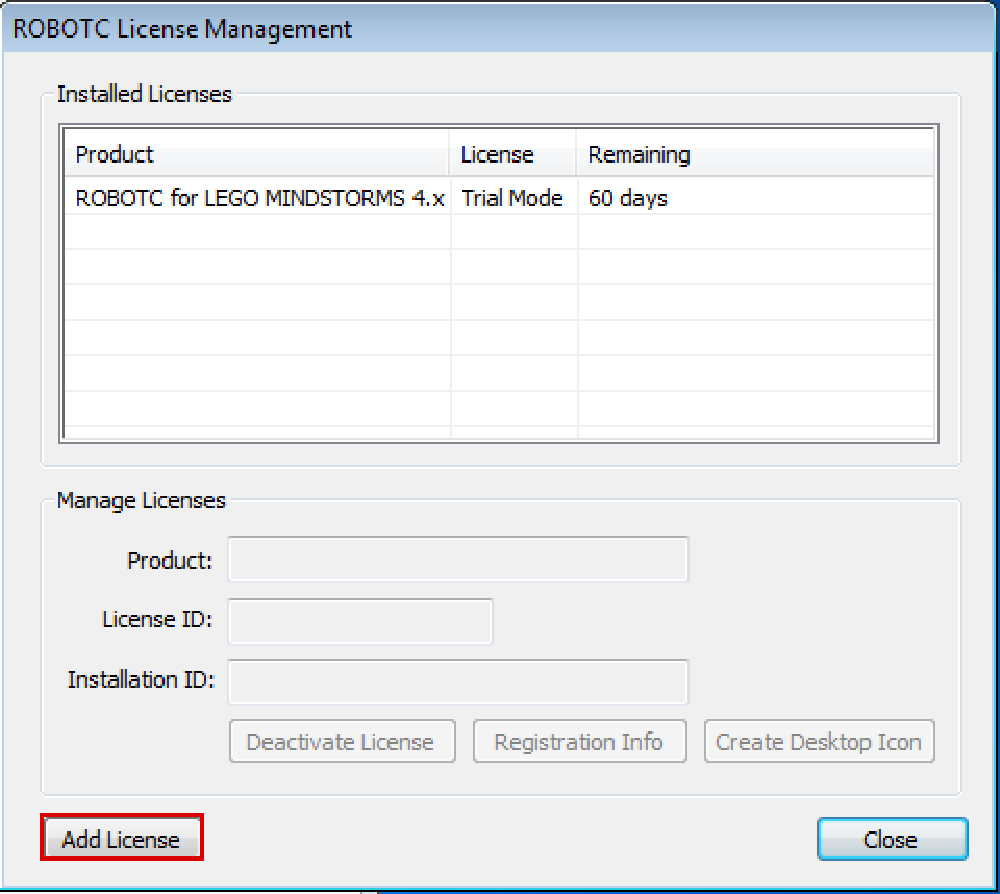
\includegraphics{2-add-license.pdf}}\\
(2) ライセンス追加\\
   \resizebox{5cm}{!}{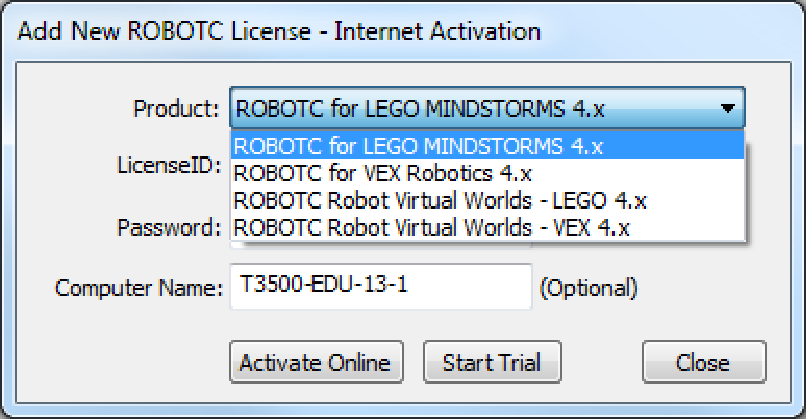
\includegraphics{3-product-license.pdf}}\\
(3) Product選択\\
   \resizebox{5cm}{!}{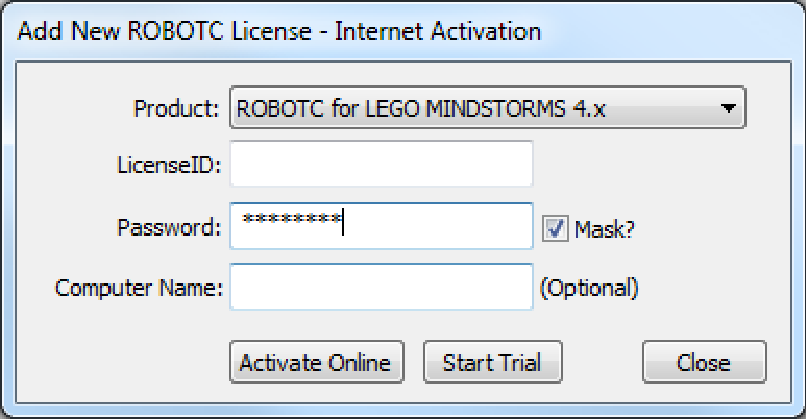
\includegraphics{4-id-license.pdf}}\\
(4) アカウント情報入力\\
}
\caption{\label{fig:activation}RobotCのアクティベーション}
\end{wrapfigure}
\subsection{演習課題について}
このテキストで\textbf{「課題」}とある箇所は,関連する質問や指示
が elearningのページにあります。\textbf{必ず回答}してください。
\textbf{「問」}とある箇所は,指示に従って設問の内容を各自考えましょう。
結果を報告する必要はありませんが,その後の課題や演習のレースプログラム
作成のために必要になることがあるので各自必ず動作確認をしましょう。

\section{RobotCの準備}
\subsection{RobotCのインストール}

演習のelearningのページに,RotobCのインストーラのダウンロードサイトのリンク情報があります。
インストーラ%(\verb|ROBOTCforLEGOMindstorms_426| といった名前)
をダウンロード・実行して,YesかNextをひたすら選択すればインストールできます。
インストール後にデスクトップに表示されるアイコン\textbf{``ROBOTC for LEGO MINDSTORMS''}をクリックすると図\ref{fig:start}のような画面がでてきます。

\subsection{RobotCのアクティベーション}
以下の手順でアクティベーションをしてください(図\ref{fig:activation})。
ただし,\textbf{大学での情報コンセントではアクティベーションできないので,各自自宅で実行してきて下さい。}(自宅でできない人は担当教員に相談)
\begin{enumerate}
	\item RobotCのメニューで"Help/Manage License"を選択
	\item 表示されるウィンドウで"Add License"を選択
	\item Productは"ROBOTC for LEGO MINDSTORMS 4.x"を選択
	\item アカウント情報を入力(elearningのページ参照)
\end{enumerate}


\section{MindStormを動かしてみよう}
\begin{wrapfigure}[12]{r}{6cm}\vspace{-.2cm}
\begin{center}
  \resizebox{5.5cm}{!}{\includegraphics{ev3.pdf}}
\end{center}
\end{wrapfigure}
\subsection{LEGO MindStorm EV3の準備}

MindStorm EV3の上部にある\textbf{Bポートに左モータが,Cポートに右モータ}
が接続されている事を確認しましょう。
次に,センサがEV3下部の各ポートに,以下のように接続されていることを確認してください。
\begin{enumerate}
\item \textbf{入力ポート$1$に\nmindex{タッチセンサ}}
\item \textbf{入力ポート$2$に\nmindex{ジャイロセンサ}}
\item \textbf{入力ポート$3$に\nmindex{カラーセンサ}}
\item \textbf{入力ポート$4$に\nmindex[ちょうおんぱせんさ]{超音波センサ}}
\end{enumerate}
% \begin{center}
%   \begin{minipage}[t]{4cm}\centering
%     \resizebox{4cm}{!}{\includegraphics{Touch.eps}}\\
%     タッチセンサ
%   \end{minipage}
%   \begin{minipage}[t]{4cm}\centering
%     \resizebox{4cm}{!}{\includegraphics{UltraSonic.eps}}\\
%     超音波センサ
%   \end{minipage}
% \end{center}

確認したら,USBケーブルでパソコンとMindStorm EV3を接続し,
MindStorm EV3を起動しましょう。
LEGO MindStorm EV3のボタンの説明は右図を参照してください。


\subsection{RobotCの設定\label{sec:bricx}}

RobotC で利用するMindStormの機種設定を行います。
RobotCの上部メニューの
\textbf{Robot→Platform Type→LEGO Mindsotrms から「LEGO Mindsotrms EV3」を選択}します。
\begin{center}
    \centering
    \resizebox{14cm}{!}{\includegraphics{robotc-config.png}}
\end{center}

次に,プログラムを書く準備のためにメニューの\textbf{File→New}を選択ししま
しょう。その後, モータやセンサについての設定を行います。
上部の\textbf{''Motors and Sensors Setup''のアイコン}を選択してください。
\begin{center}
    \centering
    \resizebox{12cm}{!}{\includegraphics{icon-motor_sensor_setup.png}}
\end{center}
かわりに,メニューの\textbf{Robot→Motors and Sensors Setup}を選択しても
同じ設定をできます。

\subsubsection{モータポートの設定\label{sec:motorport}}

\textbf{``Motors''}と書かれたタブを開いて,\textbf{motorA}
から\textbf{motorD}までの各欄を下図のように設定してください。
Name欄には,各モータの名前を\verb|leftMotor|, \verb|rightMotor|と登録
しましょう。以下のプログラムでは,各モータにこの名前を使ってアクセスし
ます。
\begin{center}
    \centering
    \resizebox{16cm}{!}{\includegraphics{motorSet.png}}
\end{center}

\work
モータポートの設定をよく確認したら,elearningの課題をしましょう。


\subsubsection{センサポートの設定\label{sec:sensorport}}

\textbf{``Sensors''}と書かれたタブを開いて,
\textbf{S1}から\textbf{S4}の各欄を以下のように設定してください。
\begin{center}
    \centering
    \resizebox{16cm}{!}{\includegraphics{sensorSet.png}}
\end{center}
Name欄には,各センサの名前をtouchSensor, gyroSensor, colorSensor,
sonarSensor と登録しましょう。以下のプログラムでは,各センサにこの名前
を使ってアクセスします。
ポートS4に接続している超音波センサの\verb|Sensor Mode|欄で選択している
\verb|Distance CM|は,対象までの距離を単位cmで計測するようにするための
設定です。

\work
センサポートの設定をよく確認したら,elearningの課題をしましょう。

\subsection{プログラムを書いてMindStormを動かす}

以下のようなプログラムを書いてみましょう。

\begin{lstlisting}
task main()
{
  setMotorSpeed(rightMotor,50);
  setMotorSpeed(leftMotor,50);
  sleep(2000);
}
\end{lstlisting}

以下の手順でプログラムを実行しましょう。
\begin{enumerate}
\item \textbf{[保存]} \quad
  プログラムを書いたら「Save」をクリックしてファイルを保存します。
  \begin{enumerate}
  \item \textbf{ファイル名は日本語不可}です。必ず\textbf{英数文字の
    み}の名前にします。 日本語を使うと,コンパイルは出来ても実行が出来なくなります。
  \item \textbf{''()''などの記号}も使えません。
\end{enumerate}
\item \textbf{[コンパイル]}\quad
  「Compile Program」(下図)をクリックします。
  このとき,プログラム名をすでに指定しているときには,プログラムは自動で上
  書き保存されます。
\item \textbf{[ロボットにダウンロード]}\quad
  「Download to Robot」(下図)をクリックします。
  \textbf{プログラムを変更したときには, この転送をお忘れ無く}。
   \begin{center}
     \resizebox{12cm}{!}{\includegraphics{icon-compile_download.png}}
   \end{center}
   \textbf{注意) EV3を初めてノートパソコンに接続したときには,ドライバの自動インストールのため,プログラムのダウンロードをできるようになるまで少し時間がかかることがあります。}
\item \textbf{[実行]}\quad
  ダウンロード後表示される「Start」ボタンをクリックすれば実行できます。
  プログラムをMindStormにダウンロードした後は,\textbf{USBケーブルをはずして
    MindStormのボタンを操作してもプログラムの実行はできます}。
\end{enumerate}

\subsection{プログラムにエラーがおきた時}
コンパイル時にエラー行に$\times$印が表示されます。
エラーの原因は下のウィンドウに表示されます。

\begin{center}
    \resizebox{8cm}{!}{\includegraphics{robotc_compile_error.pdf}}
\end{center}

プログラムが暴走したときには,\textbf{「電源ボタン」と
「戻る」ボタンを同時に押すと強制終了}できます。

\subsection{ファイルの消し方}

\textbf{演習終了時には,MindStorm上にある自分のプログラムを消去しましょう}。
RobotCの上部メニュー"Robot/LEGO Brick/File Management Utility"で,MindStorm上のファイル操作ができます。


\newpage
\section{RobotCの基本文法}

\subsection{モータを動かす}
C言語のプログラムでは必ずmain関数を一つだけ書きますが,
ROBOTCでは\verb|main()|という名前のtask(タスク)を必ず一つだけ書きます。
タスクと関数は役割が少し違いますが,それについては後述します。


\begin{lstlisting}
task main()
{
  setMotorSpeed(rightMotor,50);
  setMotorSpeed(leftMotor,50);
  sleep(2000);	//wait 2000 milliseconds
  setMotorSpeed(rightMotor,-30);
  setMotorSpeed(leftMotor,-30);
  sleep(2000);		
  setMotorSpeed(rightMotor,0);
  setMotorSpeed(leftMotor,0);
}
\end{lstlisting}
プログラム中の関数や記号の意味は以下の通りです。
\begin{itemize}
\item 各行において''\verb|//|''より後は\nmindex{コメント}とみなされます。
  C言語と同様に\verb|/* */|ではさむこともできます。
  ただし,\textbf{コメント文には日本語は使えません}。
\item \index{setMotorSpeed()}
  \verb|setMotorSpeed(port,speed)|は,指定したポート(port)に接続され
  ているモータを,指定した出力(speed [\%])で動かす命令です。
  speed は int型の$-100$から$100$の数値で指定します。
  引数portにはモータを接続しているポート番号か,\ref{sec:motorport}節で設定したモータ名を
  指定します。
  モータの回転方向を変えるには,出力の符号を変えます。
\item \index{sleep()}
  \verb|sleep(time)|は,指定した時間(time [ms])だけ次の行の命令の実行
  を待ち,それまでの命令を継続する命令です。
\end{itemize}

% \question
% 少しバックしてから向きを変えて$3$秒前進するプログラムを作りましょう。


\subsection{LCDディスプレイ表示\label{sec:LCD}}
以下はMindStorm の LCDディスプレイに文字や数値を出力するプログラム例です.

\begin{lstlisting}
task main()
{
  int i=1234;
  displayTextLine(0,"i=%d",i);
  sleep(2000);
  displayCenteredTextLine(2,"Hello World");
  sleep(2000);
  eraseDisplay();
  sleep(2000);
  displayBigTextLine(3,"Hello World");
  sleep(2000);
  displayCenteredBigTextLine(5,"i=%d",i-1000);
  sleep(2000);
}
\end{lstlisting}

上記のプログラムで使っている関数の詳細は以下の通りです.
\index{eraseDisplay()}
\index{displayTextLine()}
\index{displayCenteredTextLine()}
\index{displayBigTextLine}
\index{displayCenteredBigTextLine()}
\begin{center}
\begin{tabular}[t]{l|l}\hline
関数名 & 機能 \\\hline
\verb|eraseDisplay()| & 画面を消す\\
\verb|displayTextLine(n,string,...)| & n行目に文字stringを表示\\
\verb|displayCenteredTextLine(n,string,...)| & n行目に文字stringを中央揃えで表示\\
\verb|displayBigTextLine(n,string,...)| & n行目に文字stringを大文字で表示\\
\verb|displayCenteredBigTextLine(n,string,...)| & n行目に文字stringを大文字かつ中央揃えで表示\\\hline
\end{tabular}
\end{center}
なお,残念ながら日本語の表示はできません。

%\work
%LCDディスプレイ中央に, 1秒ごとに''3'', ``2'', ``1''とカウントダウンの数字
%を表示し,最後に自分の名前を表示するプログラムを作りなさい。


\subsection{変数の型と基本演算}
RobotCでは,C言語のように\nmindex[へんすう]{変数}を使うこともできます。
以下は利用できる変数の型の例です。

\index{bool}
\index{byte}
\index{char}
\index{float}
\index{long}
\index{int}
\index{short}
\index{string}
\index{word}
\index{ubyte}
\index{void}
\begin{quote}
  \begin{tabular}{lcr}
    \multicolumn{1}{l}{bool} & \dots 
    & \multicolumn{1}{l}{trueかfalseの二値をとる変数型} \\
    \multicolumn{1}{l}{byte} & \dots 
    & \multicolumn{1}{l}{整数型(8bit,-128$\sim$127)} \\
    \multicolumn{1}{l}{char} & \dots
    & \multicolumn{1}{l}{整数型(8bit, -128$\sim$127)} \\
    \multicolumn{1}{l}{float} & \dots
    &  \multicolumn{1}{l}{浮動小数点型(32bit)} \\
    \multicolumn{1}{l}{long} & \dots
    &  \multicolumn{1}{l}{整数型 (32bit, -2,147,483,648$\sim$2,147,483,647)} \\
    \multicolumn{1}{l}{int} & \dots
    & \multicolumn{1}{l}{整数型 (16bit, -32,768$\sim$32,767)} \\
    \multicolumn{1}{l}{string} & \dots
    & \multicolumn{1}{l}{文字型} \\
\end{tabular}
\end{quote}


数値演算のときにもC言語と同様に,
\verb|+, -, ++, --, /, &, +=, -=|などの
\nmindex[えんざんし]{演算子}を使うことができます。

\work
以下のプログラムを作成して各変数の値をMindStormのLCDディスプレイに表示
し,予想通りの値が表示されているか確認しなさい。
% 表示された値はelearningのページに回答しなさい。

\begin{lstlisting}
int a, b, c, d;

task main()
{
  a=5;
  b=2*a+1;
  b/=a;
  a%=3;
  c=++a;
  d=c++;
  displayTextLine(0,"a=%d",a);
  displayTextLine(1,"b=%d",b);
  displayTextLine(2,"c=%d",c);
  displayTextLine(3,"d=%d",d);
  sleep(2000); /* wait 2s */
}
\end{lstlisting}

% LCDディスプレイへの表示方法の詳細は\ref{sec:LCD}節を参照してください。

% \subsubsection{乱数}
% \index{random()}
% 関数\verb|random(n)|は0からnまでの整数\nmindex[らんすう]{乱数}を返します。
% 以下はプログラム例です。

% \begin{lstlisting}
% int move_time,turn_time;
% task main()
% {
%         srand(nSysTime);
%         move_time=random(1000);
%         turn_time=random(1000);

%         setMotorSpeed(rightMotor,50);
%         setMotorSpeed(leftMotor,50);
%         sleep(move_time);
%         setMotorSpeed(leftMotor,-50);
%         sleep(turn_time);
% } 
% \end{lstlisting}

% \index{srand()}
% \index{nSysTime}
% 関数\verb|srand()|は\verb|nSysTime|を引数として\textbf{乱数の初期値を
%   設定}しています。
% \verb|nSysTime|はロボットの起動時間(msec)の下16ビットの値を示す変数です。 

\subsection{関数}
\subsubsection{関数の定義}
RobotCにもC言語の関数と同様の関数(function\index{function})があります。
% 関数はタスクから呼び出す事もできますし,関数から他の関数を呼び出す事もで
% きます。
以下の例では関数の返り値は\verb|void|ですが,C言語と同様に\verb|int|や
\verb|float|等を返り値にすることもできます。

\begin{lstlisting}
void straight(int pwr)
{
  setMotorSpeed(rightMotor,pwr);
  setMotorSpeed(leftMotor,pwr);
}

task main()
{
  straight(50);
  sleep(1000);
  straight(-30);
  sleep(1000);
  straight(0);
}
\end{lstlisting}

\subsubsection{引数のアドレス渡し}
C言語と同様にポインタを使って引数の\bfindex[あどれすわたし]{アドレス渡し}を実現できます
以下はその例です。

\begin{lstlisting}
int foo(int x)
{
  static int y=2;
  x++;
  y++;
  return(y);
}

void bar(int *x)
{
  (*x)++;
}

task main()
{
  int x=1,y,z;
  y=x++;
  z=foo(y);
  displayCenteredBigTextLine(2,"x=%d",x);
  displayCenteredBigTextLine(3,"y=%d",y);
  displayCenteredBigTextLine(4,"z=%d",z);
  z=++x;
  bar(&z);
  displayCenteredBigTextLine(5,"z=%d",z);
  z=foo(y);
  displayCenteredBigTextLine(6,"z=%d",z);  
  sleep(2000);
}
\end{lstlisting}

この例では,関数fooにおいて\bfindex[せいてきへんすう]{静的変数}も使われています。

\work
上のプログラムを作成し,変数$y$の値が予想通りの値に表示されるか確認し
なさい。
% x=2, y=1, z=4

\subsubsection{引数のアドレス渡し(C++の書式)}
引数の\bfindex[あどれすわたし]{アドレス渡し}は,C++言語と同様に
関数の定義部の引数に\&をつけることで,アドレス渡しの指定をすることもできます。
以下の2つのプログラムは, 同じプログラムをCの記法とC++の記法で書いたものです。
C++の記法の場合,
関数\verb|bar|の引数定義(1行目)には\&をつけ,それ以外(
関数\verb|bar|内で引数の値を修正するとき(3行目)や,関数\verb|main|内で
関数\verb|bar|を呼び出すとき(9行目))の変数名は,通常の変数表記にすれば良いので,表記が簡潔になります。

\begin{lstlisting}
void bar(int *x) //アドレス渡しなのでポインタでアドレスを受け取る
{
  (*x)++;        //アドレスxに格納されている値(*x)を書き換える
}

task main()
{
  int x=1;
  bar(&x); // 変数のアドレスを関数barに渡す
  displayCenteredBigTextLine(5,"x=%d",x);
  sleep(2000);
}
\end{lstlisting}\begin{lstlisting}
void bar(int &x) //アドレス渡し
{
  x++;           //通常の変数と同様に書けば良い
}

task main()
{
  int x=1;
  bar(x); // アドレス渡しでも単に変数名を書くだけで良い
  displayCenteredBigTextLine(5,"x=%d",x);
  sleep(2000);
}
\end{lstlisting}

\subsubsection{配列・構造体}

\nmindex[はいれつ]{配列}や\nmindex[こうぞうたい]{構造体}もC言語と同様に利用できます。配列の各要素は$0$に初期化されます。
以下の二つのプログラムは,同じアルゴリズムを配列と構造体で作った例です。

\begin{lstlisting}
#define RIGHT 0
#define LEFT 1

void initSpeed(int *v) //値を書き換えるのでアドレス渡し
{
  v[RIGHT]=100;
  v[LEFT]=50;
}

void setSpeed(int *v) //配列を受け取るのでアドレス渡し
{
  setMotorSpeed(rightMotor,v[RIGHT]);
  setMotorSpeed(leftMotor,v[LEFT]);
}

task main() 
{ 
  int v[2];

  initSpeed(v);
  setSpeed(v);
  while(true);
} 
\end{lstlisting}

\begin{lstlisting}
typedef struct{
   int right;
   int left;
} motorSpeed;

void initSpeed(motorSpeed &v) //値を書き換えるのでアドレス渡し
{
  v.right=100;
  v.left=50;
}

void setSpeed(motorSpeed v) //構造体(値は書き換えない)だと参照渡しでOK
{
  setMotorSpeed(rightMotor,v.right);
  setMotorSpeed(leftMotor,v.left);
}

task main() 
{ 
  motorSpeed v;

  initSpeed(v);
  setSpeed(v);
  while(true);
} 
\end{lstlisting}
関数\verb|initSpeed()|では引数\verb|v|の値を書き換えるので,
引数をアドレス渡しで受取る必要があります。
%アドレス渡しはC言語のようにポインタを使うかわりに,上記のプログラムのように
%関数の引数に\verb|&|をつけることで,アドレスを受け取ることを示すことが出来ます。
%これは\verb|C++|と同じ記法です。

\subsection{制御構文}

\subsubsection{条件式}

\nmindex[ifぶん]{if文}等の\nmindex[じょうけんしき]{条件式}において
\textbf{値が非0ならば真, 0ならば偽}と判定されます。
条件式ではC言語と同様に \verb|==|, \verb|>|, \verb|<=| 等の多くの演算子
を使うことが出来ます。
\textbf{「真を表す記号」として''true''}, \textbf{「偽を表す記号」
  として''false''}を使うことも出来ます。

% \begin{center}
% \begin{tabular}{ll}  \\ \hline
% 記号 &  意味  \\ \hline
% true   &  真  \\ 
% false  &  偽  \\ \hline
% $==$  &  \verb|if(x==3){...}|\\
% $!=$  &  \verb|if(x!=y){...}| \\
% $<$    &   \\
% $<=$  &  \\
% $>$      &  \\
% $>=$   &  \\
% $!$             &  \\
% $\&\&$ &  \\ 
% $\mid\mid$    &  \\ \hline
% \end{tabular}
% \end{center}


\subsubsection{if 文,while文}
\nmindex[ifぶん]{if文}や\nmindex[whileぶん]{while文}もC言語と同様に使えます。
以下のプログラム例で,\verb|while(true)|の\verb|true|は「真」
を意味するので,while文のループ内は永久に実行され続けることになります。


\index{\#define}

\begin{lstlisting}
#define MOVE_TIME 1000
#define TURN_TIME 500

void forward(int pwr)
{
  setMotorSpeed(rightMotor,pwr);
  setMotorSpeed(leftMotor,pwr);
}

task main()
{
  srand(nSysTime);
  while(true){
    forward(50);
    sleep(MOVE_TIME);
    if(random(1) == 0){
      forward(-50);
    } else {
      setMotorSpeed(rightMotor,-50);
    }
    sleep(TURN_TIME);
  }
}
\end{lstlisting}
プログラム中の
\index{random()}
関数\verb|random(n)|は0からnまでの整数\nmindex[らんすう]{乱数}を返します。
\index{srand()}
\index{nSysTime}
関数\verb|srand()|は\verb|nSysTime|を引数として\textbf{乱数の初期値を
  設定}しています。
\verb|nSysTime|はロボットの起動時間(msec)の下16ビットの値を示す変数です。 
 
\work 上のプログラムを組んでロボットの動作をよく理解したら,elearning
の設問に答えなさい。

\subsubsection{for文\label{sec:for}}

\index{forぶん@for文}
\verb|for|文もC言語と同様に使うことが出来ます。

\begin{lstlisting} 
#define MOVE_TIME 1000
#define TURN_TIME 500

task main()
{
  for(int i=1;i<=3;i++){
    setMotorSpeed(rightMotor,50);
    setMotorSpeed(leftMotor,50);
    sleep(MOVE_TIME);
    setMotorSpeed(leftMotor,-50);
    sleep(TURN_TIME);
  }
}
\end{lstlisting}

\subsubsection{do$\sim$while文}
以下のように \nmindex[dowhileぶん]{do$\sim$while文}も使うことができます。

\begin{lstlisting}
do { 
  ...
} 
while (condition); 
\end{lstlisting}

do文ではまず\verb|do|に続く\verb|{}|内の命令を一度実行した後に,
\verb|while()|で指定した条件が評価されることに気をつけましょう。

\work \ref{sec:for}節のプログラムをdo$\sim$while文を使って書き換えなさ
い。
% 作ったプログラムはelearningのページにアップロードしなさい。

% \question
% 次のプログラムの動作を説明しなさい。

% \begin{lstlisting}
% int move_time, turn_time, total_time;
% task main()
% {
%   srand(nSysTime);
%   total_time=0;
%   do {
%     move_time=random(1000);
%     turn_time=random(1000);

%     setMotorSpeed(rightMotor,50);
%     setMotorSpeed(leftMotor,50);
%     sleep(move_time);
%     total_time+=move_time;

%     setMotorSpeed(leftMotor,-50);
%     sleep(turn_time);
%     total_time+=turn_time;
%   } while(total_time < 20000);
% }
% \end{lstlisting}

\newpage
\section{センサーを使う}

\subsection{タッチセンサを使う}

以下は何かにぶつかるまで直進するプログラム例です。

\begin{lstlisting}
void forward(int pwr)
{
  setMotorSpeed(rightMotor,pwr);
  setMotorSpeed(leftMotor,pwr);
}

task main()
{
  forward(50);
  while (getTouchValue(touchSensor)==false){}
  forward(0);
}
\end{lstlisting}

\index{getTouchValue()}
関数\verb|getTouchValue(port)|は,指定したポートに接続しているタッチセンサがなにかに接触した時には1 (true) を,接触していない時には0 (false) を返します。
引数portにはタッチセンサを接続しているポート番号か,\ref{sec:sensorport}節で設定したタッチセンサ名を指定します。


%\index{SetSensor()}
%\index{\#pragma config()}
%上のプログラム例では,\verb|SensorValue[Touch]|を,タッチセンサーが接
%続されているポート名S1を使って\verb|SensorValue[S1]|としても良いですが,
%これだとどのセンサの値かわかりにくいですね。
%そこで,このプログラムでは,\verb|#pragma config()|を用いることで
%MindStormのどの\nmindex[にゅうりょくぽーと]{入力ポート}にどのようなセ
%ンサが接続されているかを指定し,センサの名前(入力ポートの別名)を定義
%しています。


%\protect\verb|#pragma config(Sensor, 入力ポート, このセンサーにつける名前,  センサーの種類, オプション)|
%\begin{itemize}
%\item 第1引数は''Sensor''としましょう。
%\item 第2引数の入力ポートの指定はポート番号に応じて\verb|S1|から
%  \verb|S4|で行います。
%\item 第3引数は,センサにアクセスするためのセンサ名(ポート番号の
%  別名)を設定できます。
%  どのセンサーか分かりやすい名前にしましょう。
%\item 第4引数は,センサーの種類に応じて以下のいずれかを選択します。
%  \begin{itemize}
%  \item タッチセンサ: \verb|sensorEV3_Touch|
%  \item カラーセンサ: \verb|sensorEV3_Color|
%  \item 超音波センサ: \verb|sensorEV3_Ultrasonic|
%  \item ジャイロセンサ: \verb|sensorEV3_Gyro|
%  \end{itemize}
%\item 第5引数以下には,センサを利用するためのオプションを設定する
%  ことがありますが,通常は記入する必要ありません。
%\end{itemize}


以下は障害物に当たったら少し後ろに下がってから向きを変えて動き続けるプ
ログラム例です。

\begin{lstlisting}
void forward(int pwr)
{
  setMotorSpeed(rightMotor,pwr);
  setMotorSpeed(leftMotor,pwr);
}

task main()
{
  while(true){
    forward(50);
    if(getTouchValue(touchSensor)==true){
      forward(-50);
      sleep(500);
      setMotorSpeed(rightMotor,50);
      sleep(500);
    }
  }
}
\end{lstlisting}

\work
上記のプログラムに,タッチセンサが衝突を検出した回数をカウント・表示する関数を追加し, main関数から呼び出すよう修正しなさい。回数のカウントには静的変数(static)を新しく作る関数内で定義して用いること。


%\index{SensorValue[]}
%\verb|SensorValue[]|は,\textbf{さまざまなセンサからの情報を0から
%100までの数値にして格納している配列}です。
%上のプログラム中の\verb|SensorValue[Touch]|の返り値は,タッチセンサが
%物体に接触しているときには$1$(true),非接触の時には$0$(false)になります。

\subsection{カラーセンサを使う: 明るさを取得する}

カラーセンサの横にはLEDライトがついています。
LEDライトを消灯すると周囲の明るさや色情報を,
LEDライトを点灯するとその反射光によって,カラーセンサのすぐ前にある
対象の明度や色の情報を得ることが出来ます。

LEDライトの反射光から対象の明度を取得する関数には以下の2つがあります。
\begin{itemize}
\item
\index{getColorReflected()}\verb|int getColorReflected(port)|:
赤色LEDを点灯して反射光の明度を表す$0$から$100$までの数値を返します。
返り値が大きいほど明度が高いことを示します。
\item \index{getColorAmbient()}\verb|int getColorAmbient(port)|:
赤色以外のLEDを点灯して,反射光の明度を返します。
\end{itemize}
以下は地面が明るいと時計回り,暗い時には反時計回りに回転するプログラムです。
光センサの値はMindStormのLCDディスプレイに表示されます。

\begin{lstlisting}
#define THRESHOLD 40

void clockwise(long pwr)
{
  setMotorSpeed(rightMotor,-pwr);
  setMotorSpeed(leftMotor,pwr);
}

task main()
{
  int s;
  while(true){
    s=getColorReflected(colorSensor);
    displayCenteredBigTextLine(5,"Light:%d",s);
    if(s>THRESHOLD){
      clockwise(50);
    } else {
      clockwise(-50);
    }
  }
}
\end{lstlisting}


\question
上記のプログラムを改造して,カラーセンサを使って床面に描かれている黒線
の右縁に沿ってロボットを動かすライントレースのプログラムを作ってみましょ
う。
カラーセンサで取得した床面の明度はLCDに表示させるようにしてください。

\work
まっすぐ直進しながら,床面にある黒線を横切った回数を数え,4本目の黒線
を通過したところで停止するプログラムを作りなさい。黒線を横切った回数はディスプレイに表示するようにしなさい。

\subsection{カラーセンサを使う: 色情報を取得する}

\index{getColorRGB}
関数\verb|getColorRGB(port,&red,&green,&blue)|
\footnote{\&ついている引数は,ポインタを使わずにアドレス渡しを実現できることを示します。C++言語の書式と同じです。}
を使うと,カラーセンサを
使って対象の赤, 青, 緑の各色の強さを0から255の数値で知ることができます。
以下は地面の色の情報をMindStormのLCDディスプレイに表示するプログラムです。
% Sensor ModeをAmbientにしてもLEDは消えない...!?

\begin{lstlisting}
task main()
{
  long redValue;
  long greenValue;
  long blueValue;

  while (true){
    getColorRGB(colorSensor, redValue, greenValue, blueValue);
    displayCenteredBigTextLine(5,"RGB:%d,%d,%d", redValue, greenValue, blueValue);
    sleep(100);
  }
}
\end{lstlisting}

\begin{wrapfigure}[3]{r}{3cm}\vspace{-.7cm}
  \resizebox{2.6cm}{!}{\includegraphics{red-zones.pdf}}
\end{wrapfigure}
\work\label{q:go-back}
右図のように赤く塗りつぶされた2地点がある。
その一方から出発し,他方に到達したら後進してもとの場所に戻る
動作を繰り返すプログラムを作り,その動作を確認しなさい。

\begin{wrapfigure}[7]{r}{4.2cm}%\vspace{-.5cm}
\begin{center}
  \resizebox{4cm}{!}{\includegraphics{Color.eps}}\\
  旧型光センサ
\end{center}
\end{wrapfigure}
\subsection{旧型光センサを使う}

明るさのみを検出できる(色情報は取得できない)旧型(MindStorm NXT用)の光
センサを使う場合,
\textbf{\ref{sec:sensorport}節のセンサ設定}で
センサ名(Name)を\verb|lightSensor|とし,\verb|Sensor Type|は
\verb|Light-Reflected(NXT)|
% (LEDを点灯する場合),もしくは
% \verb|Light-Ambient(NXT)|(LEDを消灯する場合)
を指定して下さい。
プログラム中でLEDを消灯したい時には以下を実行します。
\begin{lstlisting}
  SensorType[lightSensor]=sensorLightInactive;
\end{lstlisting}
点灯する時には右辺を\verb|sensorLightActive|とします。

以下は,周囲の明るさを取得して表示するプログラムです。
\begin{lstlisting}
task main()
{
  while(true){
    displayCenteredBigTextLine(5,"Light:%3d",SensorValue(lightSensor));
  }
}
\end{lstlisting}

関数\index{SensorValue}\verb|SensorValue(port)|は,指定ポートのセンサ
値を0から100までの値で返します。


\subsection{超音波センサを使う}

超音波センサは,出した音が返ってくるまでの時間を計ることで前方の物体ま
での距離を測ることができるセンサです。
距離は関数\index{getUSDistance()}\verb|getUSDistance(port)|を使って単
位 cm または inch で取得できます。
どちらの単位を使うかは\ref{sec:sensorport}節で指定できます。

\question 以下のプログラムの動作を説明し,実際にロボットを使って動作確
認をしなさい。


\begin{lstlisting}
#define NEAR 15 //cm

task main()
{
  while(true){
    setMotorSpeed(rightMotor,50);
    setMotorSpeed(leftMotor,50);
    while(getUSDistance(sonarSensor) > NEAR){}
    setMotorSpeed(rightMotor,0);
    setMotorSpeed(leftMotor,-50);
    sleep(400);
  }
}
\end{lstlisting}


\work
ロボットがヒトの後ろをついてくるようなプログラムを作りたい。
ヒトの代わりに,下敷き等をロボットの前にかざして,ロボットの前後運動を
操作できるプログラムをここでは作成する。
超音波センサでロボットの前方にある物体までの距離を測り,前方の物体が動
いても常に30cm程度の距離を保つように動くことができるプログラムを作りな
さい。

\subsection{ジャイロセンサを使う}

ジャイロセンサは,回転の角速度を計測することができるセンサーです.
その積分により回転角度も得ることが出来ますが,積分により求められる
\textbf{角度は時間とともに誤差が蓄積するので注意}しましょう.
以下がジャイロセンサを用いるための関数です。
\begin{itemize}
\item
\index{getGyroDegrees()}
\verb|long getGyroDegrees(port)|: 
ジャイロセンサをMindStormに接続したとき,もしくはMindStormを起動してからの
回転角度を度数法で返す。
時計回りに回転する時にはこの値は増え,反時計回りのときは減る。
\item 
\index{resetGyro()}
\verb|void resetGyro(port)|: ジャイロセンサの初期化(現在の角度を0度と
定義し直す)をする。
上述のように,一般にジャイロセンサを用いて求めた角度には誤差が蓄積しやすいので,
MindStormがある方向を向くとわかる適当なタイミングが時々あるなら,そのタイミングで
ジャイロセンサを初期化すると良い。
\item 
\index{getGyroHeading()}
\verb|void getGyroHeading(port)|: 
最後にジャイロセンサをリセットしてからの回転角度を度数法で返す。
時計回りに回転する時にはこの値は増え,反時計回りのときは減る。
\item
\index{getGyroRatio()}
\verb|long getGyroRate(port)|: ジャイロセンサの角速度 [degree/s]を返す。
返り値は-440 degree/sから440 degree/s の値を取る。
\end{itemize}

以下はジャイロセンサを使って90度回転するブログラム例です.

\begin{lstlisting}
void rotate(int pwr)
{
  setMotorSpeed(rightMotor, -pwr);
  setMotorSpeed(leftMotor, pwr);
}

task main()
{
  resetGyro(gyroSensor);

  while(getGyroDegrees(gyroSensor) < 90){
    rotate(50);
  }

  rotate(0);
}
\end{lstlisting}


以下は,ジャイロセンサで計測した角速度に応じて進行方向を調整するプログ
ラムです.

\begin{lstlisting}
void turn_right(int power,int turn)
{
   setMotorSpeed(rightMotor, power-turn);
   setMotorSpeed(leftMotor, power+turn);
}

task main()
{
   while(true){
      long omega=getGyroRate(gyroSensor);

      if(abs(omega) > 3){
         turn_right(50,5*sgn(omega));
      } else {
         turn_right(50,0);
      }
   }
}
\end{lstlisting}

\index{sgn()}
\index{abs()}
\verb|sgn(float)|は,指定した値が正なら1を,負なら-1を,0なら0を
返す関数, \verb|abs(float)|は絶対値を返す関数です.

\question
MindStormに接続させている全てのセンサから得られる様々な値
(接触センサ,超音波センサ,光センサ(R,G,B),ジャイロセンサ(角度,角
速度))の一覧を画面に表示するプログラムを作りなさい。
センサ値は1秒ごとに更新し,
光センサで得られる明度と(R,G,B)値は1秒ごとに交互に表示するようにしなさい。

\work
課題\ref{q:go-back}と同様に赤く塗りつぶされた2地点がある。
その一方から出発し,他方に到達したところで180度回転して,もとの場所に
戻る動作を繰り返すプログラムを以下のように作り,その動作を確認しなさい。
回転角度の検出にはジャイロセンサを用いること。


\newpage
\section{並列タスク}

\index{startTask()}
RobotCには\bfindex[へいれつけいさん]{並列計算}の機能があり,複数の作業
を同時に行う事ができます。
\textbf{並列して実行する作業単位}を\bfindex{task}と呼びます。
% ロボットに,(1)何事もなければ直進,(2)ぶつかったら方向転換,という動作を
% させたい時には(1)と(2)に対応するtaskを書いて並列処理をします。
% この2つのタスクの実現に必要な実行単位(前進する,後進するなど)は関数
% にして,タスクから呼び出すことができます。
\verb|task main()|もtaskを定義する関数のひとつで,
プログラム実行時にはまずこれが呼び出されます。
他のtaskは\verb|task main()|から関数\verb|startTask()|で呼び出します。
%並列処理が不要なら\verb|task main()|以外のtaskは作らなくてもよいです。
以下は,ロボットが障害物に当たったら方向転換しながら動き回るプログラム例です。
ロボットを直進させるタスク\verb|move_forward()|と,タッチセンサ
の入力を監視しながら入力があれば方向転換をするタスク
\verb|check_touch()|を並列処理しています。

\begin{lstlisting}
TSemaphore flag;

void forward(int pwr)
{
    setMotorSpeed(rightMotor,pwr);
    setMotorSpeed(leftMotor,pwr);
}

task move_forward()
{
  while(true){
    semaphoreLock(flag);
    forward(50);
    semaphoreUnlock(flag);
  }
}

task check_touch()
{
  while(true){
    semaphoreLock(flag);
    if(getTouchValue(touchSensor) == true){
      forward(-50);
      sleep(500);
      setMotorSpeed(leftMotor,50);
      sleep(500);
    }
    semaphoreUnlock(flag);
  }
}

task main()
{
  semaphoreInitialize(flag);  //Initialize the semaphore
  startTask(move_forward);
  startTask(check_touch);

  while(true); // タスク実行をずっと続ける
}
\end{lstlisting}


複数のタスクを同時に実行していると,複数のタスクが1つのモータに異なる
方向に動くように命令を出してしまう可能性があります。 
このような問題を防ぐため,\bfindex{TSemaphore} (セマフォ,手旗信号)とい
う型の変数を使います。
上の例では,以下のようにセマフォを使っています。
\begin{enumerate}
\item \index{TSemaphore()}
3行目で\verb|TSemaphore|型の変数flagを宣言してします。
\item 
\index{semaphoreInitialize()}
タスクmainで関数\verb|semaphoreInitialize()|によりflagを初期化します。
\textbf{このようにセマフォの初期化はmainタスクで忘れずに実行}しましょ
う。
\item タスクmainでは次に, \verb|StartTask()|で2つのtaskを順に起動して
  います。この2つのtaskがセマフォflagを利用してモータの実行権の取り合
  いをします。
  先に関数\index{semaphoreLock()}\verb|semaphoreLock()|を実行した方が 
  変数flagにある値を書き込むことで,セマフォのロック状態であることを示
  し,他方がflagをロックできなくなります。
\item モータの実行が終わったときには,
  \index{semaphoreUnlock()}\verb|semaphoreUnLock()|により
  flagの値を変更することで,セマフォのロック解除を示す状態にします。
  flagがロック解除されるまで,もう一方のtaskは\verb|semaphoreLock()|できず,
  その後の命令も実行されません。
\end{enumerate}
セマフォを用いた実行権の奪い合いは\bfindex{mutex}(相互排除)
とも呼ばれ,並列計算で一般によく使われます。

\work 以下は,通常時は前進,障害物に当たったら後退して方向転換をするプ
ログラムを並列タスクを利用して作ろうとしたものです。
悪い点を指摘し,修正案を書きなさい。

\begin{lstlisting}
task check_touch()
{
  while(true){
    if(getTouchValue(touchSensor) == true){
      setMotorSpeed(rightMotor,-50);
      setMotorSpeed(leftMotor,-50);
      sleep(700);
      setMotorSpeed(rightMotor,50);
      sleep(700);
    }
  }
}
task forward()
{
  while(true){
    setMotorSpeed(rightMotor,50);
    setMotorSpeed(leftMotor,50);
    sleep(100);
  }
}
task main()
{
  startTask(check_touch);
  startTask(forward);

  while(true);
} 
\end{lstlisting}


\work
ライントレースをしながらもし何かにぶつかりそうになったら,もしくはぶつ
かったら少し後ろに下がってからランダムに方向転換してラインを探し、
ラインを見つけたらまたライントレースをするプログラムを並列タスクを利用し
て作りましょう。
障害物の検出は超音波センサとタッチセンサを使い,どちらのセンサが反応し
ても障害物を回避できるようにしましょう。

\newpage
\appendix
\section{用意されている数学関数の例\label{sec:math}}

\begin{itemize}
\item 
\index{abs()}
\verb|float abs(float x)|
 xの絶対値を返す

\item 
\index{sgn()}
\verb|short sgn(float x)|
 指定した値が正なら1を,負なら-1を,0なら0を返す.

\item 
\index{sqrt()}
\verb|float sqrt(float x)|
 xの平方根を返す

\item 
\index{sin()}
\verb|float sin(float x)|
 指定した角度x [rad]に対するsin関数の値を返す

\item 
\index{cos()}
\verb|float cos(float x)|
 指定した角度x [rad]に対するcos関数の値を返す

\item 
\index{exp()}
\verb|float exp(float x)|
 exp(x) の値を返す

\item 
\index{log()}
\verb|float log(float x)|
 log(x) の値を返す

\item 
\index{random()}
\verb|int random(int n)|
0からnまでの整数\nmindex[らんすう]{乱数}を返す。

\item 
\index{srand()}
\verb|void srand(const long x)|
乱数の初期値を設定する。例えば,\verb|srand(nSysTime)|とすると,
\verb|nSysTime|の値により乱数の初期化をする。
\verb|nSysTime|はロボットの起動時間(msec)の下16ビットの値を示す変数。

\end{itemize}

\appendix{その他}

RobotCのメニュー"View/Function Libary (Text)"を有効にすると,
RobotCで使うことができる関数や変数の一覧が表示されます。

% \begin{itemize}
% \item 
% % \index{getBatteruCurrent()}
% % \verb|float getBatteruCurrent()|
% %  バッテリーから供給されている電流量を表示する。
% \end{itemize}

\printindex
\end{document}
